\noindent

\includegraphics[height=1.25cm]{images/pictograms/replication}
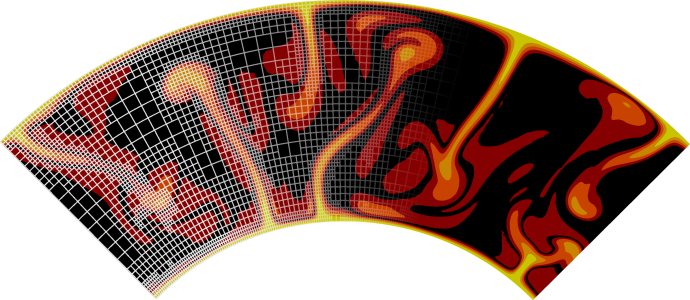
\includegraphics[height=1.25cm]{images/pictograms/aspect_logo}

\includegraphics[height=1.25cm]{images/pictograms/benchmark}

\includegraphics[height=1.25cm]{images/pictograms/FEM}
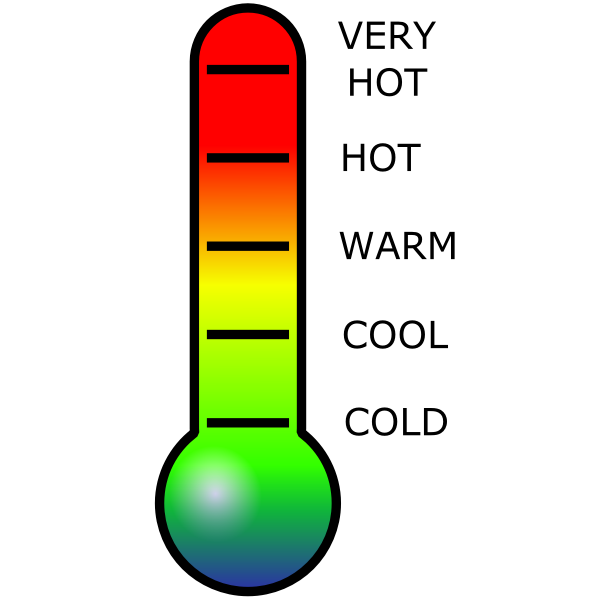
\includegraphics[height=1.25cm]{images/pictograms/temperature}

\includegraphics[height=1.25cm]{images/pictograms/3d}

\includegraphics[height=1.25cm]{images/pictograms/paraview}

%%%%%%%%%%%%%%%%%%%%%%%%%%%%%%%%%%%%%%%%%%%%%%%%%%%%%%%%%%%%%%%%%%%%%%%%%%%%%%%%%%%%%%%%%%%%%%%%%%%

\begin{flushright} {\tiny {\color{gray} python\_codes/fieldstone\_20/text.tex}} \end{flushright}

\par\noindent\rule{\textwidth}{0.4pt}

\begin{center}
\inpython
{\small Code: \url{https://github.com/cedrict/fieldstone/tree/master/python_codes/fieldstone_20}}
\end{center}

\par\noindent\rule{\textwidth}{0.4pt}

Last revision: Feb. 9th, 2025.

\par\noindent\rule{\textwidth}{0.4pt}

%%%%%%%%%%%%%%%%%%%%%%%%%%%%%%%%%%%%%%%%%%%%%%%%%%%%%%%%%%%%%%%%%%%%%%%%%%%%%%%%%%%%%%%%%%%%%%%%%%%

This three-dimensional benchmark was first proposed by \textcite{bucc94} (1994). 
It has been subsequently carried out in \textcite{tack94} (1994),
\textcite{trha98} (1998), \textcite{albe00} (2000),
\textcite{onmm06} (2006), \textcite{dawk11} (2011), \textcite{krhb12} (2012),
\textcite{thie14} (2014).
We here focus on Case 1 of the original article:  
an isoviscous bimodal convection experiment at $\Ranb=3\cdot 10^5$.

The domain is of size $a\times b\times h$ with $a=1.0079h$, $b=0.6283h$ 
with $h=\SI{2700}{\km}$. It is filled with a Newtonian fluid 
characterised by $\rho_0=\SI{3300}{\kg\per\cubic\meter}$, 
$\alpha=10^{-5}~\si{\per\kelvin}$, 
$\eta=8.0198\times10^{23}~\si{\pascal\second}$, 
$k=3.564~\si{\watt\per\meter\per\kelvin}$, 
$C_p=1080~\si{\joule\per\kelvin\per\kg}$.
The gravity vector is set to $\vec{g}=(0,0,-10)\si{\meter\per\square\second}$.
The temperature is imposed at the bottom  ($T=3700~\si{\celsius}$) and at the top ($T=0~\si{\celsius}$).

Note that using these numbers (as provided in the original paper), we arrive at $\Ranb$=29967.01, which 
is not exactly $3\cdot10^5$ as announced, although the heat diffusivity $\kappa=k/\rho_0 C_p$ is 
{\it exactly} $10^{-6}~\si{\square\meter\per\second}$.

The various measurements presented in the article are listed hereafter:
\begin{itemize}
\item The Nusselt number $\Nunb$ computed at the top surface following:
\[
\Nunb = L_z \frac{\int\int_{z=L_z} \frac{\partial T}{\partial y} dx dy  }{\int \int_{z=0} T dx dy}.
\]
\item The root mean square velocity $\upnu_{rms}$ and the temperature mean square velocity $T_{rms}$.
\item The vertical velocity $w$ and temperature $T$ at points $\vec{r}_1=(0,0,L_z/2)$, 
$\vec{r}_2=(L_x,0,L_z/2)$, $\vec{r}_3=(0,L_y,L_z/2)$ and $\vec{r}_4=(L_x,L_y,L_z/2)$.
\item The vertical component of the heat flux $Q$ at the top surface  at all four corners. 
\end{itemize}

\begin{center}
\includegraphics[height=6cm]{python_codes/fieldstone_20/images/krhb12}
\includegraphics[height=6cm]{python_codes/fieldstone_20/images/elefant}\\
{\captionfont Left: 
Velocity field and isosurfaces of the temperature at steady state obtained 
with \aspect.\\ Taken from \textcite{krhb12} (2012).
Right: same, obtained with \elefant \cite{thie14}.}
\end{center}


\noindent Given the dimensions of the domain, here are resolutions that would yield (roughly) cubic elements:
\begin{center}
\begin{tabular}{l|lccccccc|}
domain size & \\
\hline
$a$=1.0079$\times$2700km & nelx= &16 &20 &24 &28 &32 &36 &40 \\  
$b$=0.6283$\times$2700km & nely= &10 &13 &15 &18 &20 &23 &25 \\
$h$=1.0000$\times$2700km & nelz= &16 &20 &24 &28 &32 &36 &40 \\  
\hline
\end{tabular}
\end{center}
Note that \lstinline{nelz} must be a multiple of four since we need to carry out measurements at 
locations characterised by $z=3L_z/4$.

%............................
\subsection*{Methodology}

In what follows I highlight a few important points which are key to understanding how the code
is put together and works. 

\begin{verbatim}
load needed modules and functions
define parameters
build V grid (xV,yV,zV)
build V connectivity (iconV)
define b.c. for velocity (bc_fixV,bc_valV)
build T grid (xT,yT,zT)
build T connectivity (iconT)
define b.c. for temperature (bc_fixT,bc_valT)
initial temperature field
.------------------------> istep ---------------------.
|  build K,G,f,h                                      |
|  assemble them in A,rhs                             |
|  solve                                              |
|  split solution vector in u,v,w,p                   |
|  {u,v,w}=relax*{u,v,w}+(1-relax)*{u,v,w}            |
|  compute vrms                                       |
|  build A, rhs for temperature                       |
|  solve for temperature T                            |
|  T=relax*T+(1-relax)*T                              |
|  compute elemental strainrate                       |
|  compute nodal strainrate                           |
|  compute nodal pressure                             |
|  measure V and T at mid side edges, Nu ...          |
|  export to vtu and ascii files                      | 
.---------------------------<-------------------------.
\end{verbatim}

I fist load the shape functions which are in two separate files:

\begin{lstlisting}
from shape_functionsV import NNV,dNNVdr,dNNVds,dNNVdt
from shape_functionsT import NNT,dNNTdr,dNNTds,dNNTdt
\end{lstlisting}
Technically these are the same functions since the polynomial space for 
both velocity (components) and temperature is $Q_2$.

There are \lstinline{NV=nnx*nny*nnz} velocity nodes and 
\lstinline{NT=NV} temperature nodes.

The velocity grid is built: \lstinline{xV, yV, zV, iconV}, and 
these are copied in \lstinline{xT, yT, zT, iconT} for the temperature grid.  

The initial temperature field is built as follows:
\begin{lstlisting}
for i in range(0,NT):
   T[i]= (Temperature2-Temperature1)/Lz*zT[i]+Temperature1 \
       + 100*(np.cos(np.pi*xT[i]/Lx) + np.cos(np.pi*yT[i]/Ly))*np.sin(np.pi*zT[i]/Lz)
\end{lstlisting}

The ${\bm C}$ matrix of Eq.~\eqref{MMM-eq:mixedC} is then built:
\begin{lstlisting}
c_mat = np.array([[2,0,0,0,0,0],\
                  [0,2,0,0,0,0],\
                  [0,0,2,0,0,0],\
                  [0,0,0,1,0,0],\
                  [0,0,0,0,1,0],\
                  [0,0,0,0,0,1]],dtype=np.float64) 
\end{lstlisting}

%.......................................
\subsubsection{Getting to steady state}  

In this case we are not so much interested in the path to steady state since 
the published values/measurements are {\it at} steady state.
The mass and momentum conservation equations for incompressible Stokes flow do not 
contain a time derivative but the energy conservation equation does. 

At steady state the terms $\partial_t T$ is zero by definition so we must solve
the following equation\footnote{Adiabatic heating, shear heating and internal heating 
are not considered in the benchmark} (see Section~\ref{MMM-ss:hte}):
\begin{equation}
\vec{\upnu}\cdot\vec\nabla T - {\vec \nabla} \cdot k {\vec \nabla} T = 0
\end{equation}
The Finite Element discretisation of this equation yields 
\[
({\bm K}_a + {\bm K}_d) \cdot \vec{T} = \vec{b}
\]
where $\vec{b}$ contains the boundary conditions.
This formulation is much simpler than the time-dependent one and avoids to discuss the choice
of time-discretisation algorithm altogether. 

We now have to solve three coupled equations:
\begin{eqnarray}
-{\vec \nabla}p + {\vec \nabla}\cdot (2 \eta \dot{\bm \varepsilon}^d ) + \rho(T) {\vec g} &=& \vec{0} \\
{\vec \nabla}\cdot{\vec \upnu} &=& 0 \\ 
\vec{\upnu}\cdot\vec\nabla T - {\vec \nabla} \cdot k {\vec \nabla} T &=& 0 
\end{eqnarray}
We could then proceed to write the weak forms of these equations and cast these as we have done before, 
but this time considering velocity, pressure and temperature as unknowns of a (very) large system:
\[
\left(
\begin{array}{ccc}
\K & \G & . \\
\G^T & 0 & . \\
. & . & . 
\end{array}
\right)
\cdot
\left(
\begin{array}{c}
\vec{\cal V} \\ \vec{\cal P} \\ \vec{\cal T}
\end{array}
\right)
=
\left(
\begin{array}{c}
. \\ . \\ .
\end{array}
\right)
\]
Once this matrix is filled a single solve will yield the steady state velocity, pressure and 
temperature fields! 

The term $\rho(T)$ will naturally end up in the (1,3) block of the assembled matrix as matrix ${\bm L}$.
The mass conservation equation in this form is independent of temperature so the (2,3) block 
will be zero. The diffusion term ${\bm K}_d$ naturally finds its way to the (3,3) 
block and since there is not occurence of pressure in the energy equation the (3,2) 
block will be zero. We then obtain:
\[
\left(
\begin{array}{ccc}
\K & \G & {\bm L} \\
\G^T & 0 & 0 \\
. & 0 & {\bm K}_d 
\end{array}
\right)
\cdot
\left(
\begin{array}{c}
V \\ P \\ T 
\end{array}
\right)
=
\left(
\begin{array}{c}
. \\ . \\ .
\end{array}
\right)
\]
The last remaining term is the advection term of the energy equation and it is a problematic one:
it features the product of the velocity by the temperature. As such it is nonlinear and one cannot 
either put it in the (3,1) block nor in the (3,3) block. 

This approach fails, which is why 
the problem is solved iteratively. The idea is simple: when solving the 
coupled mass and momentum equations, we assume temperature known, and when solving the energy equation
we assume velocity known. We can then alternatively solve one system and then the other, constantly 
updating the fields when re-building the matrices or right hand sides.

However, it is well known that a straightforward implementation of this algorithm does not 
work in practice, i.e. it fails to converge, which is why a relaxation scheme is often implemented:
\begin{enumerate}
\item Solve for velocity and pressure
\item relax velocity
\begin{lstlisting}
u=relax*u+(1-relax)*u_old
v=relax*v+(1-relax)*v_old
w=relax*w+(1-relax)*w_old
\end{lstlisting}
\item Solve for temperature
\item relax temperature
\begin{lstlisting}
T=relax*T+(1-relax)*T_old
\end{lstlisting}
\item check for convergence:
\begin{lstlisting}
if np.abs(Nu-Nu_old)<1.e-5:
   break
\end{lstlisting}
\item store old fields
\begin{lstlisting}
u_old=u
v_old=v
w_old=w
T_old=T
\end{lstlisting}
\end{enumerate}
The relaxation parameter \lstinline{relax} should be between 0 and 1.
In this case I found that a relaxation coefficient of 1 actually works.
Note that at the moment the same coefficient is used to relax both velocity and temperature, I have 
not explored different values for both.

%........................................
\subsubsection*{Computing nodal derivatives}  

Another interesting approach here is how the strain rate is computed on the nodes as well as
the temperature gradient. The strain rate is not needed for the required measurements of this 
benchmark but the Nusselt number calculations require $\partial T/\partial z$ at the top
boundary.    
The idea is simple: loop over all elements, and for each element loop over its support nodes
(in this case the $2\times 2\times 2$ nodes of the $Q_1$), compute the required derivative 
there and add its contribution to the nodal field. Finally divide the obtained field by 
the number of elements each node is part of.

\begin{lstlisting}
    for iel in range(0,nel):
        for i in range(0,mV):
            [...]
            for k in range(0,mV):
                dT_dx += dNNNVdx[k]*T[iconV[k,iel]]
                dT_dy += dNNNVdy[k]*T[iconV[k,iel]]
                dT_dz += dNNNVdz[k]*T[iconV[k,iel]]
            # end for
            dTdxn[iconV[i,iel]]+=dT_dx
            dTdyn[iconV[i,iel]]+=dT_dy
            dTdzn[iconV[i,iel]]+=dT_dz
            c[iconV[i,iel]]+=1.
        # end for i
    # end for iel
    dTdxn/=c
    dTdyn/=c
    dTdzn/=c
\end{lstlisting}

%........................................
\subsubsection*{Jacobian estimates}  

Because the mesh is regular and all elements have the same size $h_x,h_y,x_z$
then the Jacobian of the transformation from an element to the reference element
is given by 
\[
{\bm J}=\left( \begin{array}{ccc}
h_x/2 & 0 & 0 \\
0 & h_y/2 & 0 \\
0 & 0 & h_z/2
\end{array} \right)
\qquad
|{\bm J}|=\frac{h_xh_yh_z}{8}
\]
Since these quantities are typically evaluated at all quadrature points 
there is a substantial CPU time save by precomputing these quantities only 
once before entering the matrix building loop:

\begin{lstlisting}
jcob=hx*hy*hz/8
jcbi=np.zeros((ndim,ndim),dtype=np.float64)
jcbi[0,0]=2/hx ; jcbi[0,1]=0    ; jcbi[0,2]=0
jcbi[1,0]=0    ; jcbi[1,1]=2/hy ; jcbi[1,2]=0
jcbi[2,0]=0    ; jcbi[2,1]=0    ; jcbi[2,2]=2/hz
\end{lstlisting}


\newpage
%.......................
\subsection*{Results}

Given how the code is written and how costly 3D simulations are in general, high resolution
cases take a long time to run, even using relaxation instead of time stepping. 
From the following figures it is obvious that the value of the relaxation parameter 
does not influence the final steady state value and that using a high value close or 
equal to one is probably the best option (0.9 seems to be best in this case). 

\begin{center}
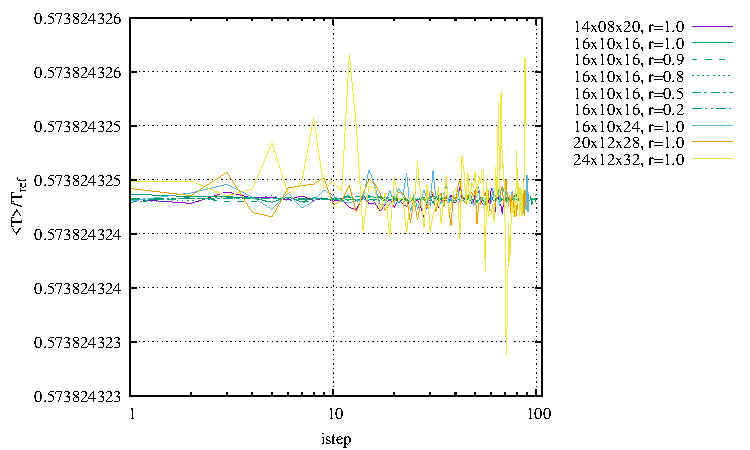
\includegraphics[width=7.5cm]{python_codes/fieldstone_20/results/Tavrg.pdf}\\
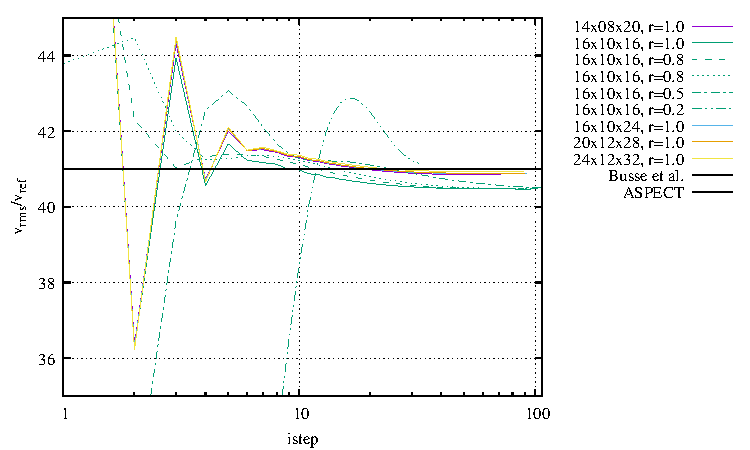
\includegraphics[width=7.5cm]{python_codes/fieldstone_20/results/vrms.pdf}
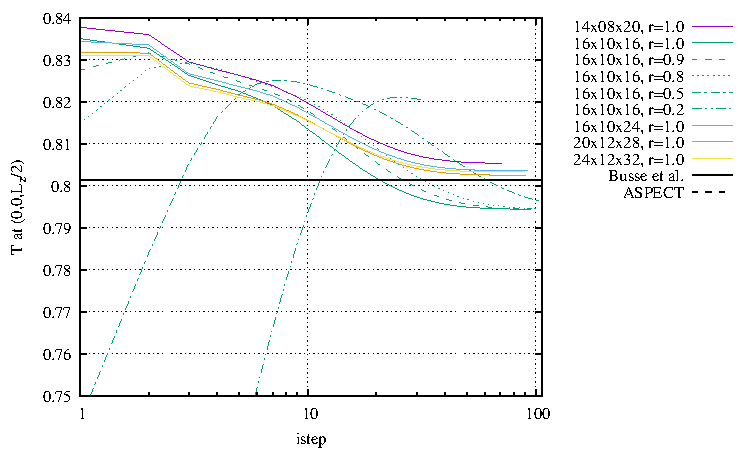
\includegraphics[width=7.5cm]{python_codes/fieldstone_20/results/Tmid.pdf}\\
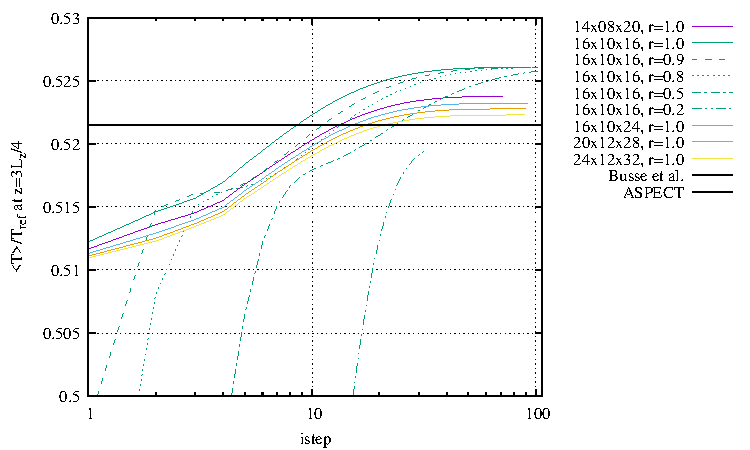
\includegraphics[width=7.5cm]{python_codes/fieldstone_20/results/Tm.pdf}
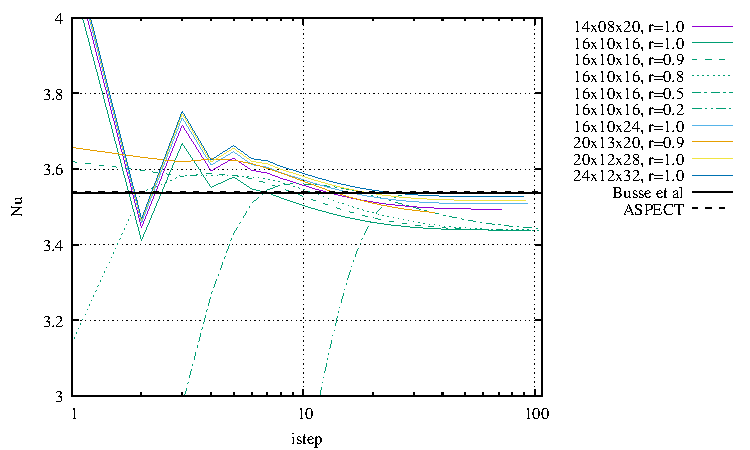
\includegraphics[width=7.5cm]{python_codes/fieldstone_20/results/Nu.pdf}\\
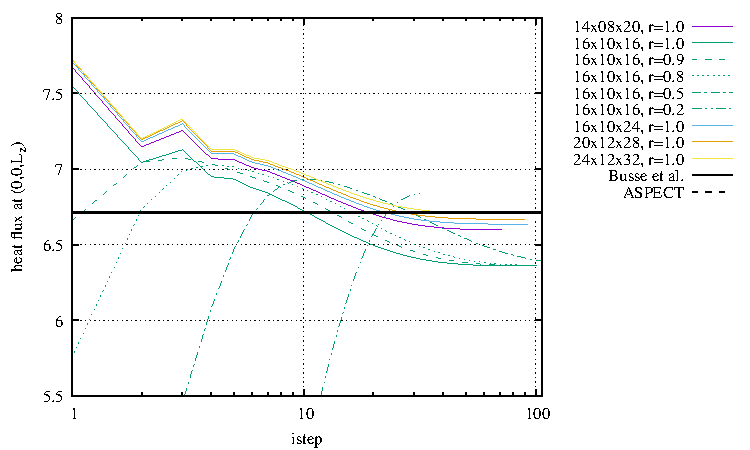
\includegraphics[width=7.5cm]{python_codes/fieldstone_20/results/hf1.pdf}
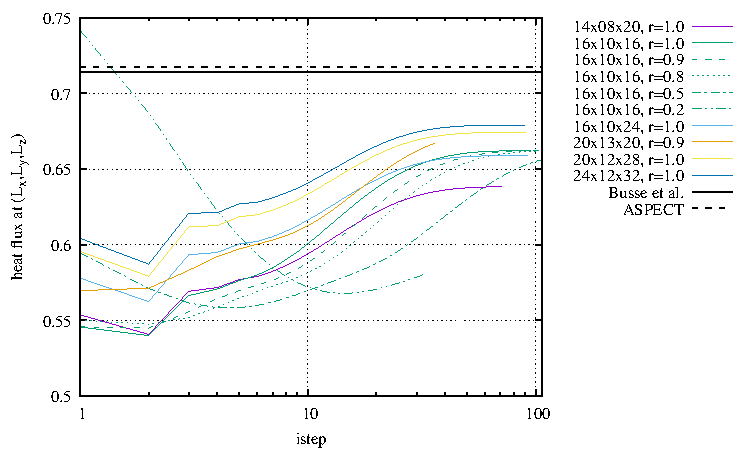
\includegraphics[width=7.5cm]{python_codes/fieldstone_20/results/hf2.pdf}\\
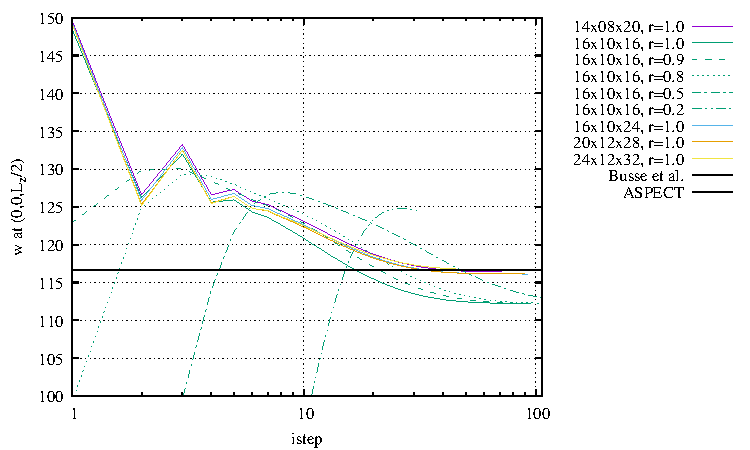
\includegraphics[width=7.5cm]{python_codes/fieldstone_20/results/wmid1.pdf}
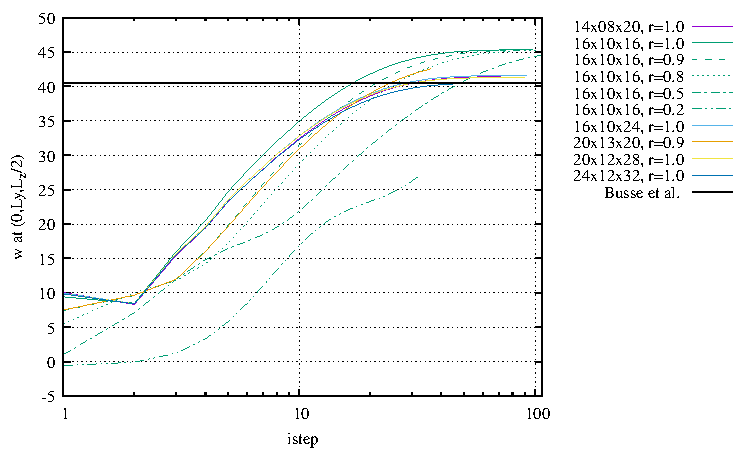
\includegraphics[width=7.5cm]{python_codes/fieldstone_20/results/wmid2.pdf}
\end{center}

\newpage
The reported values for Busse et al. in the following table are taken from Table 3 
of \textcite{bucc94} (1994).
The reported values for fieldstone are adimensionalised by means of a reference temperature (3700K),
a reference lengthscale 2700km, and a reference time $L_z^2/\kappa\sim 7.29e+18$s.
%The steady state is arrived at by solving the steady state Stokes and temperature equations 
%with a relaxation parameter of 1/2.
%To find the steady state, we simulate the problem up to non-dimensional time $t=5$, 
%i.e. $t=3.645e+19$s.


\begin{center}
\begin{tabular}{llllll}
\hline
                                & \aspect & ($Q_2\times Q_1/Q_2$)      &       & Busse et al \cite{bucc94} &  \\
Mesh size                       & Lz/24  & Lz/32 & Lz/48 & (best results)            & \\ 
\hline
$\Nunb$                         & 3.5539 &3.5447 & 3.5397 & $3.5374  \pm 0.0005$   \\
$v_{rms}$                       & 40.997 &40.999 &40.999  & $40.999  \pm 0.004$    \\
$\langle T\rangle$ at $0.75*Lz$ & 0.52148 & 0.52148&0.52148  & $0.52148 \pm 0.00003$  \\
$w(0,0,L_z/2)$     & 116.605 & 116.618 &  116.623  & $116.625 \pm 0.030$ \\
$w(L_x,0,L_z/2)$   & - &-&-& -\\
$w(L_x,L_y,L_z/2)$ & - &-&-& -\\
$w(0,L_y,L_z/2)$   &  &&& $40.500 \pm 0.030$ \\

$T(0,0,L_z/2)$     &  0.80126 & 0.80128 & 0.80129 & $0.80130 \pm 0.00005$ \\
$T(L_x,0,L_z/2)$   &  -&-&-& -\\
$T(L_x,L_y,L_z/2)$ &  -&-&-& -\\
$T(0,L_y,L_z/2)$   &  &&& $0.61876 \pm 0.00005$ \\
$dTdz(0,0,L_z)$    & 6.7679 & 6.7357 & 6.7189 & $6.7127 \pm 0.0500$ \\
$dTdz(L_x,0,L_z)$  &  & & & $1.5080 \pm 0.0500$ \\
$dTdz(L_x,L_y,L_z)$& 0.7237 & 0.7205 & 0.7174 & $0.7140 \pm 0.0500$ \\
$dTdz(0,L_y,L_z)$  &  & & & $3.1740 \pm 0.0500$ \\
\hline
\end{tabular}
\end{center}

\begin{center}
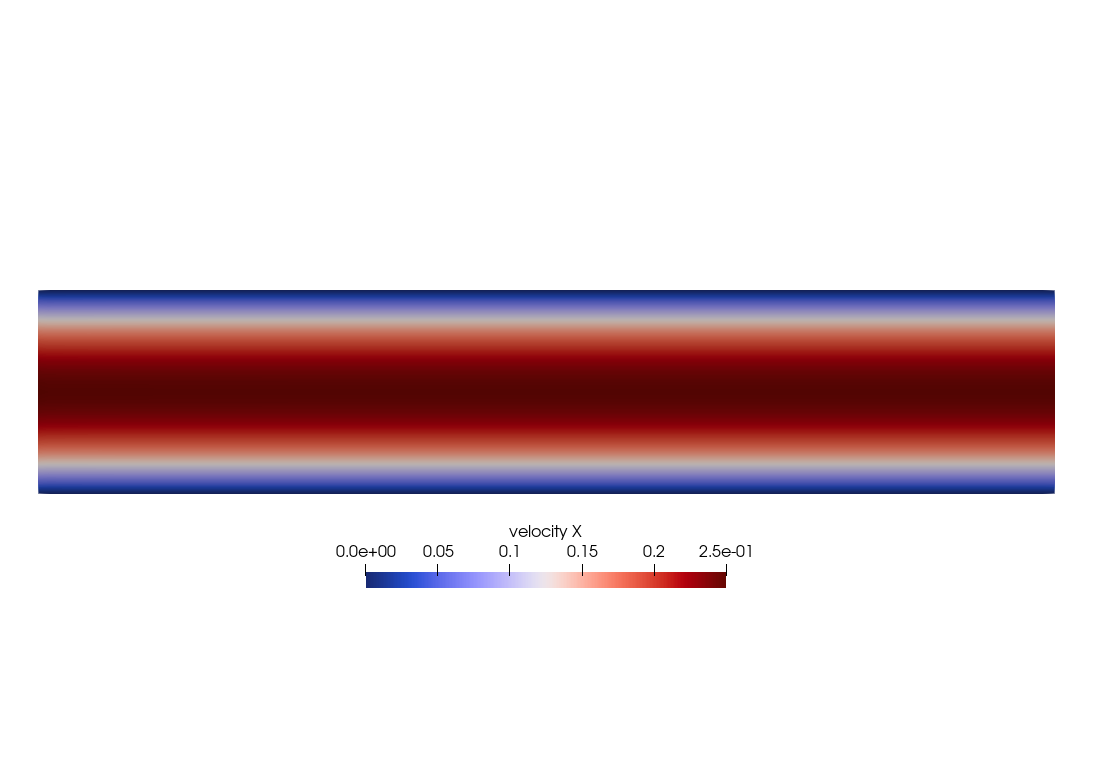
\includegraphics[width=5.5cm]{python_codes/fieldstone_20/results/24x12x32_1p0/u}
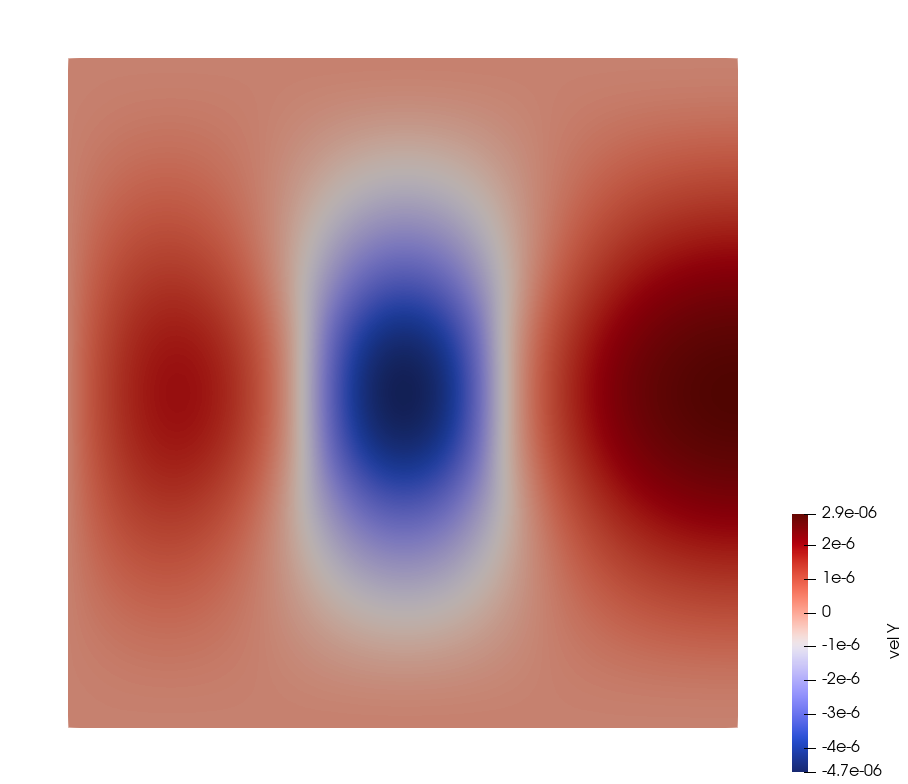
\includegraphics[width=5.5cm]{python_codes/fieldstone_20/results/24x12x32_1p0/v}
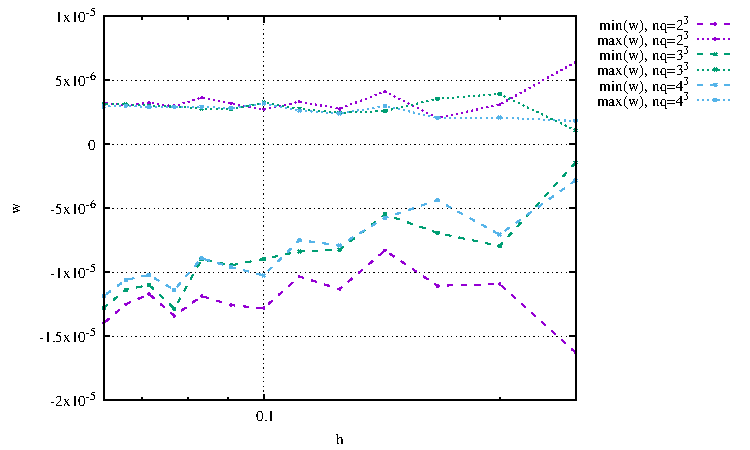
\includegraphics[width=5.5cm]{python_codes/fieldstone_20/results/24x12x32_1p0/w}\\
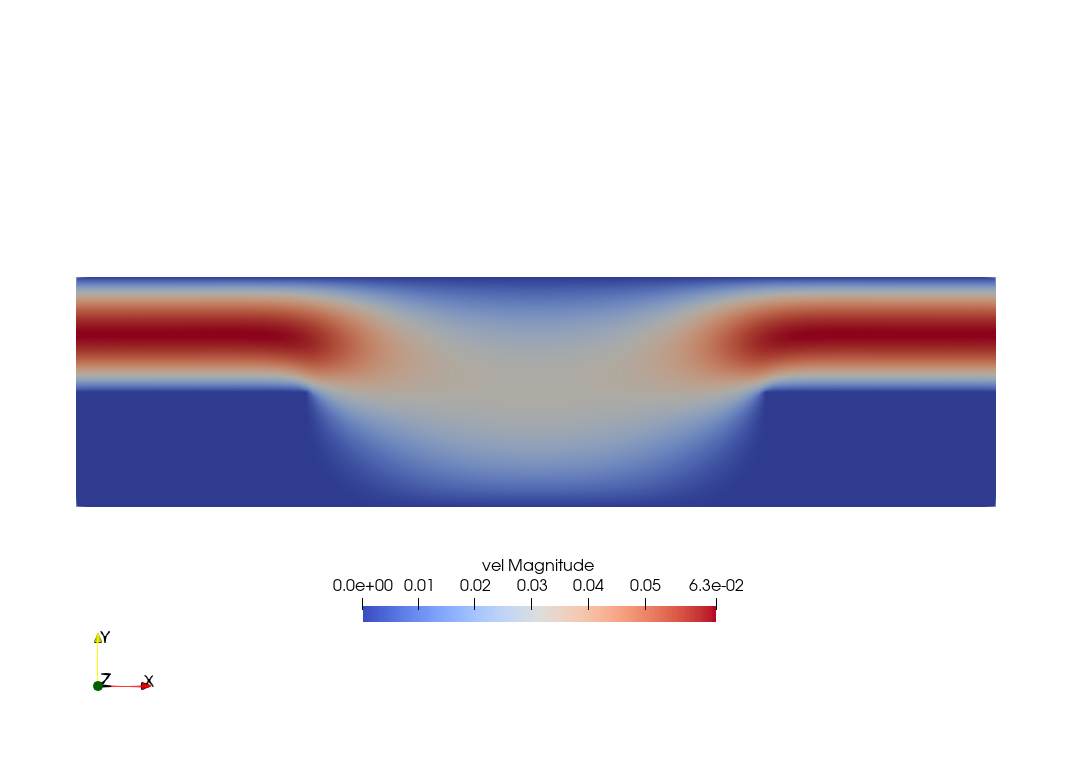
\includegraphics[width=5.5cm]{python_codes/fieldstone_20/results/24x12x32_1p0/vel}
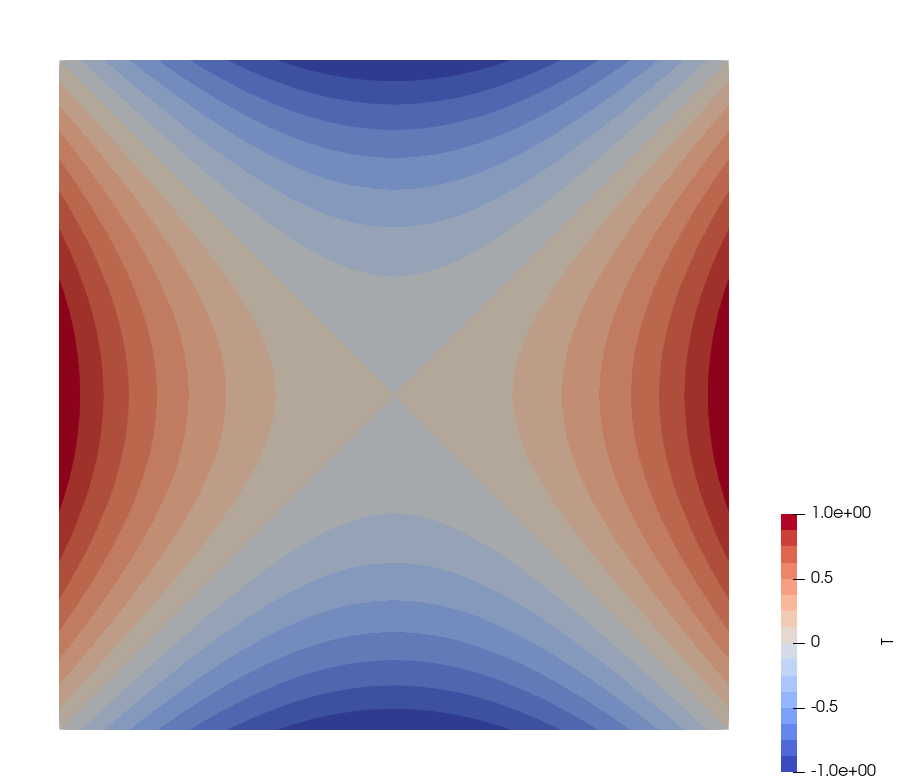
\includegraphics[width=5.5cm]{python_codes/fieldstone_20/results/24x12x32_1p0/T}
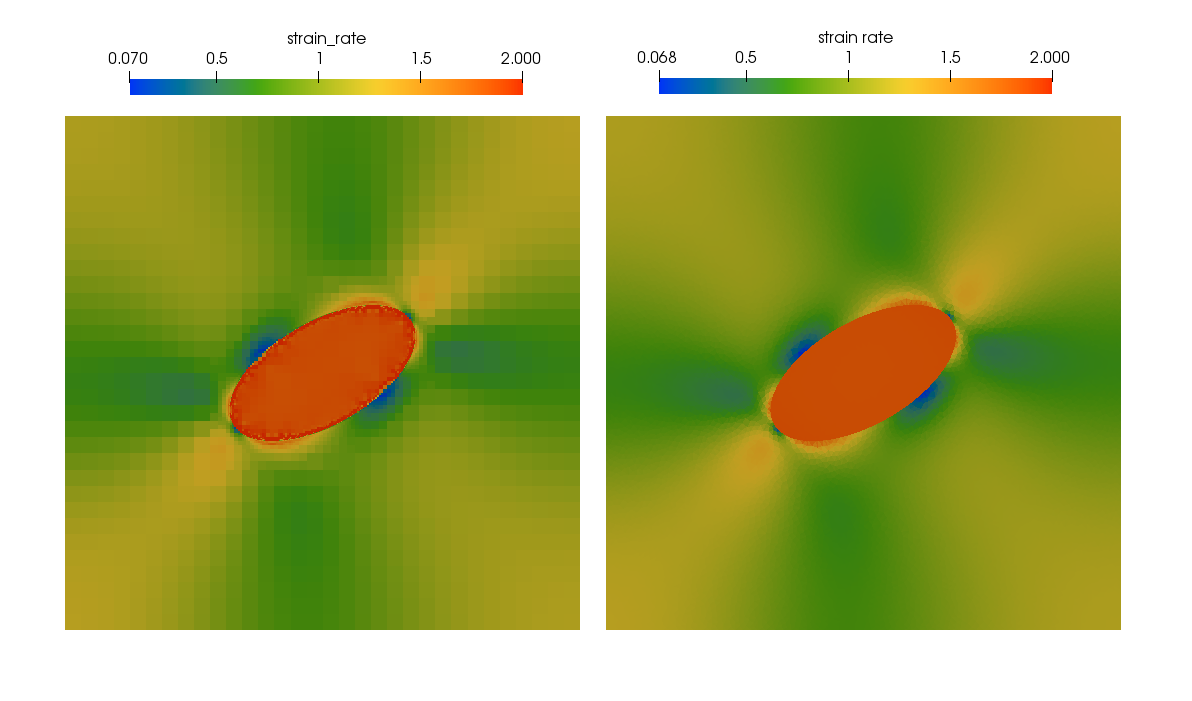
\includegraphics[width=5.5cm]{python_codes/fieldstone_20/results/24x12x32_1p0/sr}\\
{\captionfont Results obtained on $24\times 12\times 32$ mesh}
\end{center}


